\documentclass[12pt]{article}
\usepackage[utf8]{inputenc} % Pacote para acentuação gráfica
%\usepackage[T1]{fontenc}
\usepackage[brazil]{babel} % nomes das estruturas em pt-br
%\usepackage{hyperref}
\usepackage{indentfirst} % indenta primeiro paragráfo após título
\usepackage{setspace} % pacote para alterar espaçamento entre linhas
%\setlength{\parindent}{1cm} % define o tamanho da indentação
%\setlength{\parskip}{0.3cm} % define o espaçamento vertical entre parágrafos
\usepackage[top = 2cm, left = 2cm, bottom = 2cm, right = 2cm]{geometry} % define as margens do documento
\usepackage{fancyhdr} % pacote para numeração de páginas
\usepackage{lipsum}  % Pacote para gerar texto de preenchimento
\usepackage{xcolor} % Definindo novas cores
\usepackage{graphicx} % para inserir figuras
\usepackage{float} % Força o posicionamento da figura



\definecolor{verde}{rgb}{0.25,0.5,0.35}
\definecolor{jpurple}{rgb}{0.5,0,0.35}
% Configurando layout para mostrar codigos Java
\usepackage{listings}
\lstset{
	language=Python,
	basicstyle=\ttfamily\small,
	keywordstyle=\color{jpurple}\bfseries,
	stringstyle=\color{red},
	commentstyle=\color{verde},
	morecomment=[s][\color{blue}]{/**}{*/},
	extendedchars=true,
	showspaces=false,
	showstringspaces=false,
	numbers=left,
	numberstyle=\tiny,
	breaklines=true,
	backgroundcolor=\color{cyan!10},
	breakautoindent=true,
	captionpos=b,
	xleftmargin=0pt,
	tabsize=4
}
\pagestyle{empty}

\begin{document}
	
\title{\textbf{{\Huge Notas em Computação Quântica}}} % Título
\author{\textbf{{\Large Ricardo Alvarenga}}} % Autor
\date{\textbf{{\Large 2024}}} % Data
\maketitle % Criar
\thispagestyle{empty} % oculta número da página
\newpage

\pagestyle{fancy}
\setcounter{page}{1} % reset contador de página
\pagenumbering{Roman}  % Altera número de página para números romanos
\tableofcontents % cria sumário
\newpage

\listoffigures % lista de figuras
\newpage


\pagestyle{fancy}
\fancyfoot[C]{\thepage} % Adiciona o número da página no centro do rodapé
\newpage

\setcounter{page}{1} % reset contador de página
\pagenumbering{arabic}
\pagestyle{fancy}
\fancyfoot[C]{\thepage}

% \twocolumn  % Inicia o ambiente de duas colunas

\section{Álgebra Linear}

\subsection{Vetores}

Vetores são seguimentos orientados (início em 0, 0) que estão sempre no plano cartesiano. Vetores são usados para representar grandezas escalares (massa, pressão, etc.) e grandezas físicas vetoriais (velocidade, força e deslocamento).

\begin{figure}[H]
	\centering
	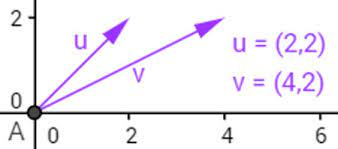
\includegraphics[width=.5\linewidth]{figuras/vetores_01}
	\caption[Vetores \textbf{u} e \textbf{v}]{Exemplos de Vetores, \textbf{u} e \textbf{v}}
	\label{fig:vetores01}
\end{figure}

\subsubsection{Vetores com duas dimensões - \( \mathbf{R}^{2} \)}

\textbf{x}, \textbf{y} podem assumir qualquer valor \textit{Real}.

\begin{figure}[H]
	\centering
	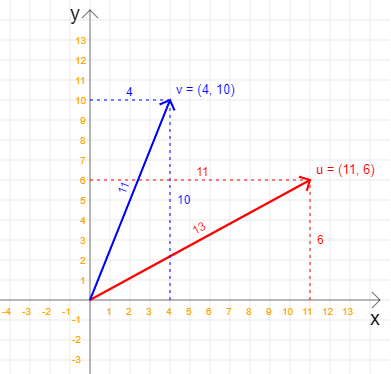
\includegraphics[height=.45\textheight]{figuras/vetores_02}
	\caption[Vetores em \( \mathbf{R}^{2} \)]{Vetores em \( \mathbf{R}^{2} \) (x, y)}
	\label{fig:vetores02}
\end{figure}

\newpage

\subsubsection{Vetores com três dimensões - \( \mathbf{R}^{3} \)}

\textbf{x}, \textbf{y}, \textbf{z} podem assumir qualquer valor \textit{Real}.

\begin{figure}[H]
	\centering
	\includegraphics[width=0.5\linewidth]{"figuras/vetores R3"}
	\caption[Vetores em \( \mathbf{R}^{3} \)]{Vetores em \( \mathbf{R}^{3} \) (x, y, z)}
	\label{fig:vetores-r3}
\end{figure}

\subsubsection{Vetores com \textit{n} dimensões - \( \mathbf{R}^{n} \)}

Os vetores com \textit{n} dimensões são de difícil (ou impossível) representação gráfica.

Um vetor \( \mathbf{R}^{4} \) é indicado da seguinte forma: \( \mathbf{R}^{4} \)(x, y, z, w)

\subsubsection{Como colocar um vetor no plano \( \mathbf{R}^{3} \)(x, y, z)}

Vetor \textbf{u} = (2,4,3)

\begin{figure}[H]
	\centering
	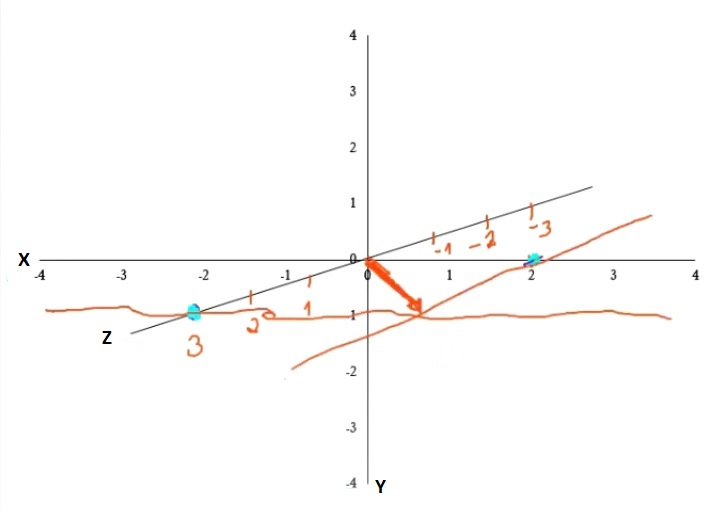
\includegraphics[width=0.7\linewidth]{figuras/R3}
	\caption[Vetor em \( \mathbf{R}^{3} \)]{Vetor em \( \mathbf{R}^{3} \)}
	\label{fig:vetor r3}
\end{figure}

\subsubsection{Tipos de Vetores}

\begin{itemize}
	\item Vetor Nulo: Todos valores iguais a zero. Ex: \textbf{v} = (0,0,0)
	\item Vetor simétrico ou oposto: Ocorre quando dois vetores são opostos e contêm o mesmo módulo e mesma direção. Ex: \textbf{v} = (x,y), \textbf{-v} = (-x,-y)
	\item Vetor unitário: Possui módulo (tamanho) igual a 1. |\textbf{v}| = 1
	\item Vetores colineares ou paralelos: Ocorrem quando dois vetores tiverem a mesma direção, na mesma reta ou retas paralelas.
	\item Vetores coplanares: Quando dois vetores fazem parte de um mesmo plano.
		
\end{itemize}

\subsubsection{Igualdade de Vetores}

Dois vetores serão iguais se: 

\begin{itemize}
	\item \(x_{1} = x_{2}\)
	\item \(y_{1} = y_{2}\)
	\item \(z_{1} = z_{2}\) vetores em \(R^{3}\)
	\item \(w_{1} = w_{2}\) vetores em \(R^{4}\)	
	\item \(u = (3, x + 4)\) \(v = (3, 8)\) se x = 4 os vetores serão iguais.
\end{itemize}

Sejam: \(u = (x-1, 3)\), \(v = (3, 2y-1)\). Determine o valor de \(x\) e \(y\) para que \(u = v\).\\

\(x = 4\), \(y = 2\)

\subsubsection{Subtração de Vetores}

\(A = (-1, 2)\)   \(B = (2,1)\)\\

\(v = $\overrightarrow{AB}$\) o vetor está "perdido" no plano cartesiano. Para corrigir isso, realizamos a subtração:\\

\(B - A = (2, 1) - ( -1, 2) = (3, -1)\)\\

Que resulta no vetor \(t = (3, -1)\), conforme figura \ref{fig:subtracaovetores01}.\\

Outro exemplo: Dois vetores \(u = (-1, 3)\) e \(v = (10, 20)\), a subtração \(u - v\) resulta em \((-11, -17)\).\\

Sejam \(u\) e \(v\) vetores no \( \mathbf{R}^{n}\)\cite{lipschutz-algebra}: \(u=(u_{1}, u_{2},...,u_{n})\) e \(v=(v_{1}, v_{2},...,v_{n})\)

\(u-v = (u_{1} - v_{1}, u_{2}-v_{2},...,u_{n}-v_{n})\).

\begin{figure}
	\centering
	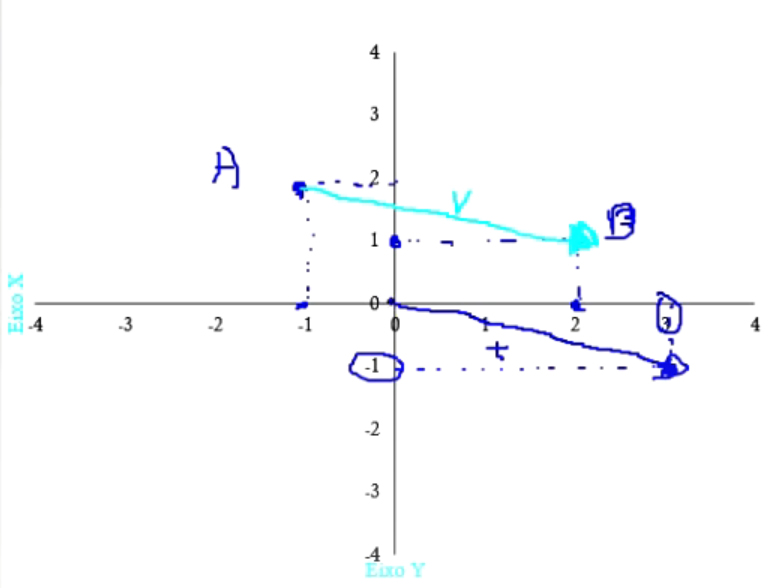
\includegraphics[width=0.7\linewidth]{figuras/subtracao_vetores_01}
	\caption[Subtração de Vetores]{Subtração de Vetores}
	\label{fig:subtracaovetores01}
\end{figure}

\pagebreak
\subsubsection{Soma de Vetores}

Assim como na subtração, temos que efetuar a soma de cada elemento com seu correspondente.\\

Exemplo:\\

\(u = (2, 3)\), \(v = (5, 6)\)\\

\(u + v = (7, 9)\)\\

\subsubsection{Produto Escalar dos Vetores (Multiplicação)}
\subsubsection{Módulo de Um Vetor}
\subsubsection{Ângulo de Dois Vetores}
\subsubsection{Paralelismo e Ortogonalidade de Dois Vetores}
\subsubsection{Projeção Ortogonal Entre Dois Vetores}

% \lipsum[1-10]  % Exemplo de texto de preenchimento

\newpage
%Biblioteca
\bibliographystyle{abbrv} %estilo
\bibliography{./referencias/referencias}
	
\end{document}